\documentclass[12pt]{article}

\usepackage{tikz} % картинки в tikz
\usepackage{microtype} % свешивание пунктуации
\usepackage{array} % для столбцов фиксированной ширины
\usepackage{comment} % для комментирования целых окружений
\usepackage{indentfirst} % отступ в первом параграфе

\usepackage{sectsty} % для центрирования названий частей
\allsectionsfont{\centering}

\usepackage{amsmath, amssymb, amsthm, amsfonts} % куча стандартных математических плюшек

\usepackage[top=2cm, left=1cm, right=1cm, bottom=2cm]{geometry} % размер текста на странице
\usepackage{lastpage} % чтобы узнать номер последней страницы
 
\usepackage{enumitem} % дополнительные плюшки для списков
%  например \begin{enumerate}[resume] позволяет продолжить нумерацию в новом списке

\usepackage{caption} % подписи к рисункам
\usepackage{hyperref} % гиперссылки
\usepackage{multicol} % текст в несколько столбцов


\usepackage{fancyhdr} % весёлые колонтитулы
\pagestyle{fancy}
\lhead{Введение в машинное обучение, ВШЭ}
\chead{}
\rhead{2022-06-24}
\lfoot{Вариант $\Sigma \Theta \Kappa$}
\rfoot{Паниковать запрещается!}
%\rfoot{Тест}
\renewcommand{\headrulewidth}{0.4pt}
\renewcommand{\footrulewidth}{0.4pt}

\usepackage{ifthen} % для написания условий

\usepackage{todonotes} % для вставки в документ заметок о том, что осталось сделать
% \todo{Здесь надо коэффициенты исправить}
% \missingfigure{Здесь будет Последний день Помпеи}
% \listoftodos --- печатает все поставленные \todo'шки


% более красивые таблицы
\usepackage{booktabs}
% заповеди из докупентации:
% 1. Не используйте вертикальные линни
% 2. Не используйте двойные линии
% 3. Единицы измерения - в шапку таблицы
% 4. Не сокращайте .1 вместо 0.1
% 5. Повторяющееся значение повторяйте, а не говорите "то же"


\usepackage{fontspec}
\usepackage{polyglossia}

\setmainlanguage{russian}
\setotherlanguages{english}

% download "Linux Libertine" fonts:
% http://www.linuxlibertine.org/index.php?id=91&L=1
\setmainfont{Linux Libertine O} % or Helvetica, Arial, Cambria
% why do we need \newfontfamily:
% http://tex.stackexchange.com/questions/91507/
\newfontfamily{\cyrillicfonttt}{Linux Libertine O}

% Математические шрифты 
% Математические шрифты 
\usepackage{unicode-math}     
\setmathfont[math-style=upright]{euler.otf} 

\setmathfont[range={\mathbb, \mathop, \heartsuit, \angle, \smile, \varheartsuit}]{Asana-Math.otf}

\AddEnumerateCounter{\asbuk}{\russian@alph}{щ} % для списков с русскими буквами
\setlist[enumerate, 2]{label=\asbuk*),ref=\asbuk*}


% мои цвета https://www.artlebedev.ru/colors/
\definecolor{titleblue}{rgb}{0.2,0.4,0.6} 
\definecolor{blue}{rgb}{0.2,0.4,0.6} 
\definecolor{red}{rgb}{1,0,0.2} 
\definecolor{green}{rgb}{0,0.6,0} 
\definecolor{purp}{rgb}{0.4,0,0.8} 

% цвета из geogebra 
\definecolor{litebrown}{rgb}{0.6,0.2,0}
\definecolor{darkbrown}{rgb}{0.75,0.75,0.75}

% Гиперссылки
\usepackage{xcolor}   % разные цвета

\usepackage{hyperref}
\hypersetup{
  unicode=true,           % позволяет использовать юникодные символы
  colorlinks=true,        % true - цветные ссылки
  urlcolor=blue,          % цвет ссылки на url
  linkcolor=black,          % внутренние ссылки
  citecolor=green,        % на библиографию
  breaklinks              % если ссылка не умещается в одну строку, разбивать её на две части?
}

% эпиграфы
\usepackage{epigraph}
\setlength\epigraphwidth{.5\textwidth}
\setlength\epigraphrule{0pt}

% Математические операторы первой необходимости:
\DeclareMathOperator{\sgn}{sign}
\DeclareMathOperator*{\argmin}{arg\,min}
\DeclareMathOperator*{\argmax}{arg\,max}
\DeclareMathOperator{\Cov}{Cov}
\DeclareMathOperator{\Var}{Var}
\DeclareMathOperator{\Corr}{Corr}
\DeclareMathOperator{\E}{\mathop{E}}
\DeclareMathOperator{\Med}{Med}
\DeclareMathOperator{\Mod}{Mod}
\DeclareMathOperator*{\plim}{plim}

\DeclareMathOperator{\logloss}{logloss}
\DeclareMathOperator{\softmax}{softmax}

\DeclareMathOperator{\tr}{tr}

% команды пореже
\newcommand{\const}{\mathrm{const}}  % const прямым начертанием
\newcommand{\iid}{\sim i.\,i.\,d.}  % ну вы поняли...
\newcommand{\fr}[2]{\ensuremath{^{#1}/_{#2}}}   % особая дробь
\newcommand{\ind}[1]{\mathbbm{1}_{\{#1\}}} % Индикатор события
\newcommand{\dx}[1]{\,\mathrm{d}#1} % для интеграла: маленький отступ и прямая d

% одеваем шапки на частые штуки
\def \hb{\hat{\beta}}
\def \hs{\hat{s}}
\def \hy{\hat{y}}
\def \hY{\hat{Y}}
\def \he{\hat{\varepsilon}}
\def \hVar{\widehat{\Var}}
\def \hCorr{\widehat{\Corr}}
\def \hCov{\widehat{\Cov}}

% Греческие буквы
\def \a{\alpha}
\def \b{\beta}
\def \t{\tau}
\def \dt{\delta}
\def \e{\varepsilon}
\def \ga{\gamma}
\def \kp{\varkappa}
\def \la{\lambda}
\def \sg{\sigma}
\def \tt{\theta}
\def \Dt{\Delta}
\def \La{\Lambda}
\def \Sg{\Sigma}
\def \Tt{\Theta}
\def \Om{\Omega}
\def \om{\omega}

% Готика
\def \mA{\mathcal{A}}
\def \mB{\mathcal{B}}
\def \mC{\mathcal{C}}
\def \mE{\mathcal{E}}
\def \mF{\mathcal{F}}
\def \mH{\mathcal{H}}
\def \mL{\mathcal{L}}
\def \mN{\mathcal{N}}
\def \mU{\mathcal{U}}
\def \mV{\mathcal{V}}
\def \mW{\mathcal{W}}

% Жирные буквы
\def \mbb{\mathbb}
\def \RR{\mbb R}
\def \NN{\mbb N}
\def \ZZ{\mbb Z}
\def \PP{\mbb{P}}
\def \QQ{\mbb Q}

\def \putyourname{\fbox{
    \begin{minipage}{42em}
      Фамилия, имя, номер группы:\vspace*{3ex}\par
      \noindent\dotfill\vspace{2mm}
    \end{minipage}
  }
}

\def \checktable{

  \vspace{5pt}
  Табличка для проверяющих работу:

\vspace{5pt}

  \begin{tabular}{|m{2cm}|m{1cm}|m{1cm}|m{1cm}|m{1cm}|m{1cm}|m{1cm}|m{1cm}|m{2cm}|}
\toprule
    Вопрос & 11 &  12 & 13 & 14 & 15 & 16 & 17 & Итого \\
\midrule
    Баллы &  &  & & & & & &  \\
 \bottomrule
\end{tabular}
}


\def \testtable{

\vspace{5pt}
  Внесите сюда ответы на тест:

\vspace{5pt}

\begin{tabular}{|m{2cm}|m{0.6cm}|m{0.6cm}|m{0.6cm}|m{0.6cm}|m{0.6cm}|m{0.6cm}|m{0.6cm}|m{0.6cm}|m{0.6cm}|m{0.6cm}|}
\toprule
    Вопрос & 1 &  2 & 3 & 4 & 5 & 6 & 7 & 8 & 9 & 10 \\
\midrule
    Ответ &  &  & & & & & & & & \\
 \bottomrule
\end{tabular}
}


% [1][3] 1 = one argument, 3 = value if missing
% эта магия создаёт окружение answerlist
% именно в окружении answerlist записаны варианты ответов в подключаемых exerciseXX
% просто \begin{answerlist} сделает ответы в три столбца
% если ответы длинные, то надо в них руками сделать
% \begin{answerlist}[1] чтобы они шли в один столбец
\newenvironment{answerlist}[1][3]{
\begin{multicols}{#1}

\begin{enumerate}[label=\fbox{\emph{\Alph*}},ref=\emph{\alph*}]
}
{
\item Нет верного ответа.
\end{enumerate}
\end{multicols}
}

% BB: unicol version. don't know why \ifthenelse fails in second part of new-env
\newenvironment{answerlistu}{
\begin{enumerate}[label=\fbox{\emph{\Alph*}},ref=\emph{\alph*}]
}
{
\item Нет верного ответа.
\end{enumerate}
}


\excludecomment{solution} % without solutions

\theoremstyle{definition}
\newtheorem{question}{Вопрос}

\usepackage{tikzlings}
\usepackage{tikzducks}

\usepackage{alltt}

\begin{document}

\putyourname

\testtable

\checktable

\mbox{ }

\epigraph{«Если орел — я выиграла, если решка — ты проиграл»
}{\textit{Рейчел Грин, сериал "Друзья"}}

Работа состоит из трёх частей: тестовая, задачи и ответы на открытые вопросы. Работа пишется на раздаточном материале. Черновики можно использовать, но не сдавать - их не проверяем.
Списывание карается обнулением работы. Удачи!

\section*{Часть первая: тестовая} 

Дайте ответ на $10$ тестовых вопросов. Каждый вопрос стоит $3$ балла. Никаких дополнительных пояснений в этой части работы от вас не требуются.

\begin{question}
Для решения задачи регрессии не подходит алгоритм
\begin{answerlist}
  \item решающего дерева.
  \item случайного леса.
  \item логистической регрессии.
  \item градиентного бустинга.
  \item KNN.
\end{answerlist}
\end{question}

\begin{solution}
\begin{answerlist}
  \item Good answer :)
  \item Bad answer :(
  \item Bad answer :(
  \item Bad answer :(
  \item Bad answer :(
\end{answerlist}
\end{solution}



\begin{question}
Джоуи не делится едой! Жадность ли это, мы не узнаем, а что верно для жадного построения дерева?
\begin{answerlist}
  \item Если разбиение сделано, оно не может быть изменено.
  \item Признаки выбираются случайно для разбиения узла.
  \item Дерево строится, пока не останется по 1 объекту в листьях.
  \item Дерево строится, пока не останутся объекты одного класса в листьях.
  \item Признаки выбираются из случайного подмножества.
\end{answerlist}
\end{question} 

\newpage

\begin{question}
Посчитайте хаотичность разбиения вершины. В качестве критерия информативности используйте критерий Джини.
    \begin{center}
        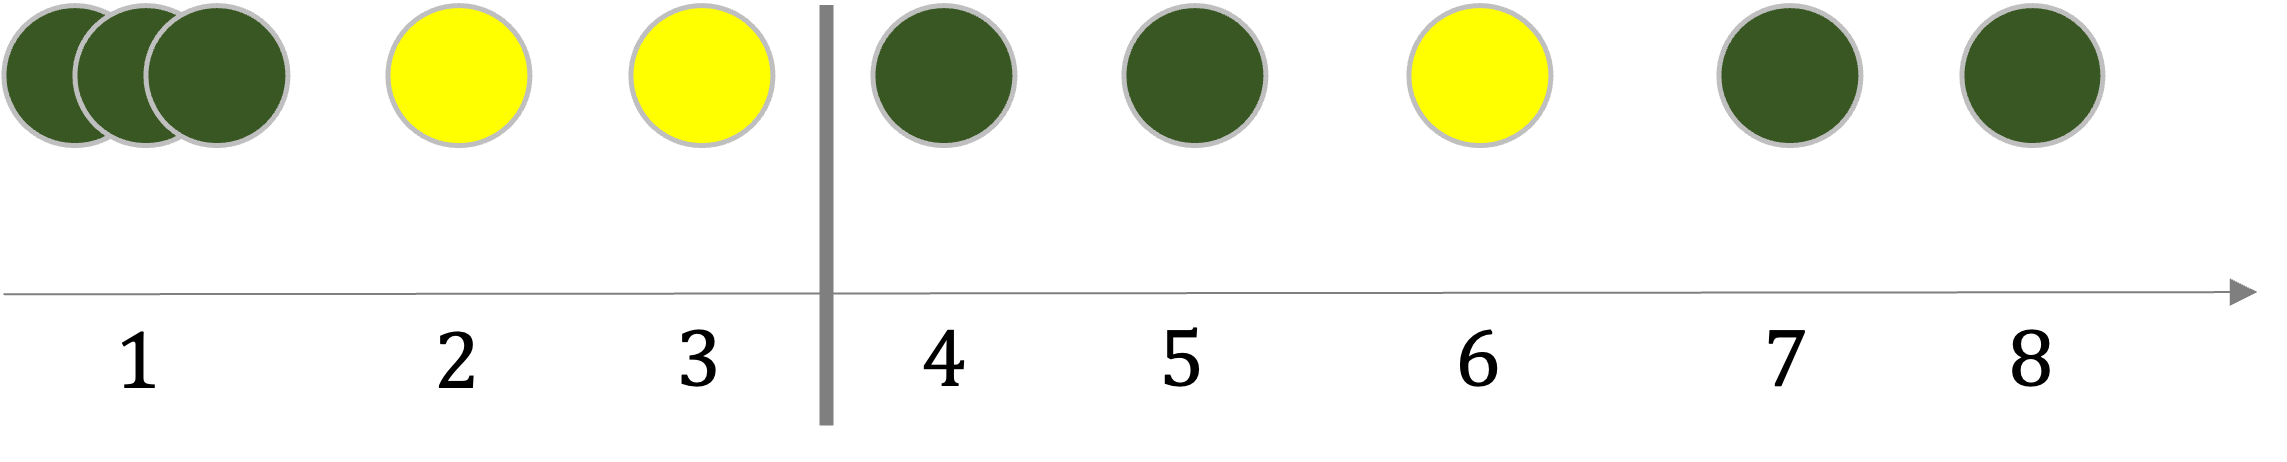
\includegraphics[scale=0.5]{entropy_var1.png}
    \end{center}
\begin{answerlist}
  \item 0.08
  \item 0.16
  \item 0.12
  \item 0.4
  \item 0.24
\end{answerlist}
\end{question}



\begin{question}
Росс прогнозирует возраст останков динозавра. Обучает градиентный бустинг. Композиция из N - 1 модели оценила в 10.5 млн лет, хотя настоящий возраст - примерно 11 млн лет. Если Росс используется MAE в качестве функции потерь, то на какой таргет будет обучаться N-ная модель?
\begin{answerlist}
  \item +1
  \item -1
  \item 0.5
  \item -0.5
  \item -1.5
\end{answerlist}
\end{question}

\begin{question}
Какой алгоритм не склонен к переобучению при увеличении соответствующего гиперпараметра?
\begin{answerlist}
  \item Решающее дерево (глубина дерева).
  \item Случайный лес (количество деревьев).
  \item Градиентный бустинг (количество деревьев).
  \item KNN (количество соседей).
\end{answerlist}
\end{question}

\begin{question}
Какого гиперпараметра нет у случайного леса?
\begin{answerlist}
  \item Max Depth.
  \item N Estimators.
  \item Learning Rate.
  \item Max Features.
  \item Min Samples Split.
\end{answerlist}
\end{question}


\begin{question}
Чендлер делает отчеты в экселе и решил изучить кластеризацию. На одном из шагов получилось такое распределение по кластерам. Где будет новый центр кластеров по координате $x$? Выберите правильную пару чисел.
\begin{table}[h]
    \centering
    \begin{tabular}{>{\bfseries}cccccccc}
        \toprule
         кластер & $1$ & $1$ & $1$ & $2$ & $2$ & $2$ \\ \midrule
         $x$ & $-1.5$ & $0.5$ & $2$ & $-1$ & $4$ & $6$\\
         \bottomrule
    \end{tabular}
\end{table}
\begin{answerlist}
  \item 0.5 и 4.
  \item -1 и 3.
  \item 3 и 9.
  \item 0.5 и 9.
  \item 4 и 9.
\end{answerlist}
\end{question}

\newpage

\begin{question}
Фиби, Рейчел, Моника и Дженис собираются на девичник. Девушки описали свои предпочтения по двум характеристикам, которые представлены в таблице. Чьи вектора интересов ближе друг к другу? Используйте косинусное расстояние как меру схожести.

\begin{table}[h]
    \centering
    \begin{tabular}{>{\bfseries}cccccccc}
        \toprule
        Имя & $x_1$ & $x_2$ \\ \midrule
         Моника & $3$ & $4$ \\ 
         Рейчел & $5$ & $12$ \\
         Фиби & $6$ & $8$ \\
         Дженис & $8$ & $15$
    \end{tabular}
\end{table}
\begin{answerlist}
  \item Моника и Рейчел.
  \item Моника и Фиби.
  \item Рейчел и Дженис.
  \item Рейчел и Фиби.
  \item Фиби и Дженис.
\end{answerlist}
\end{question}

\begin{question}
Выберите задачу, которую однозначно можно отнести к обучению с учителем.
\begin{answerlist}
  \item Понижение размерности.
  \item Кластеризация.
  \item Классификация.
  \item Рекомендательные системы.
  \item SVD.
\end{answerlist}
\end{question}

\begin{question}
Какое количество кластеров надо выбрать, судя по графику?
    \begin{center}
        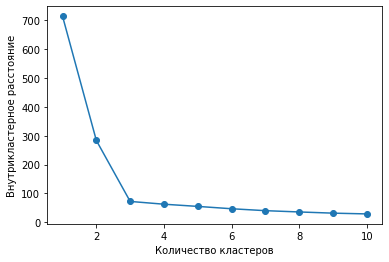
\includegraphics[scale=0.5]{elbow_method.png}
    \end{center}
\begin{answerlist}
  \item 2.
  \item 3.
  \item 4.
  \item 7.
  \item 10.
\end{answerlist}
\end{question}



\newpage 

\section*{Часть вторая: открытые вопросы}

Эта часть состоит из открытых вопросов. На них необходимо дать краткие, но ёмкие ответы. За каждый ответ вы можете получить до 10 баллов.

\begin{question}
Рассмотрим обучающую выборку для прогнозирования $y$ с помощью $x$ и $z$:
\begin{center}
    \begin{tabular}{ccc}
        \toprule
        $y_i$ & $x_i$ & $z_i$ \\
        \midrule
        $y_1$ & $1$ & $2$ \\
        $y_2$ & $1$ & $2$ \\
        $y_3$ & $2$ & $2$ \\
        $y_4$ & $2$ & $1$\\
        $y_5$ & $2$ & $1$ \\
        $y_6$ & $2$ & $1$ \\
        $y_7$ & $2$ & $1$ \\
        \bottomrule
    \end{tabular}
\end{center}

Будем называть деревья разными, если они выдают разные прогнозы на обучающей выборке. Сколько существует разных классификационных деревьев  для текущего набора данных? Изобразите их. 
\end{question}

\vspace{7cm} 

\begin{question}
Опишите пошагово, как обучается случайный лес, в том числе алгоритм построения дерева.  Объясните, что такое out of bag ошибка.
\end{question}

\newpage


\begin{question}
Рейчел сходила на свидание с доктором Митчеллом и услышала про загадочную болезнь ALS*. Она ничего не запомнила, поэтому просит помочь и описать, что это такое - ALS. Начинайте с самого начала: как ставится задача для применения этого алгоритма, что нужно сделать, какая функция потерь оптимизируется, какие шаги работы алгоритма.


(* ALS  - Amyotrophic lateral sclerosis, все совпадения случайны)
\end{question}



\newpage



\begin{question}

Джоуи готовится к роли профессора по компьютерным наукам и учит текст. По сценарию он должен объяснить своим студентам, почему использовать K-means для таких данных - плохая затея, а затем расскажет, какой алгоритм нужно использовать. Объясните, почему k-means не стоит использовать для этих данных. Предложите альтернативный алгоритм и подробно опишите, как он работает.

\begin{center}
    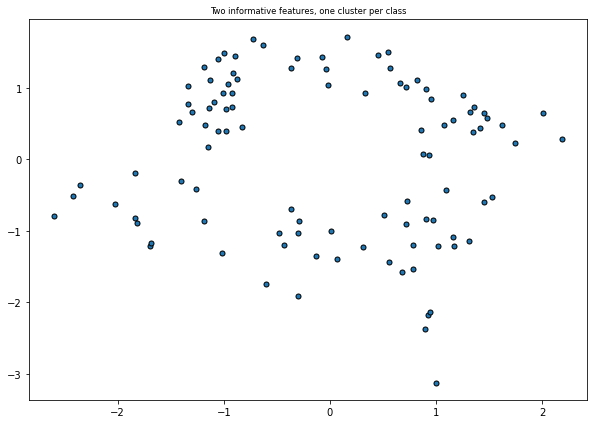
\includegraphics[scale=0.5]{clustering_var1.png}
\end{center}
\end{question}
\vspace{8cm} 







\newpage 

\begin{question}
Пока Моника ждет оффера в Twins Garden, она изучает машинное обучение. На картинке представлены 4 случайных леса, обученных Моникой на одних и тех же данных. Варьируется один гиперпараметр. Какой гиперпараметр это может быть? Предположите, какие значения гиперпараметра могут соответствовать каждой картинке. К чему приводит очень большое значение этого гиперпараметра? Предположите, какое значение и картинку стоит выбрать.
\begin{center}
    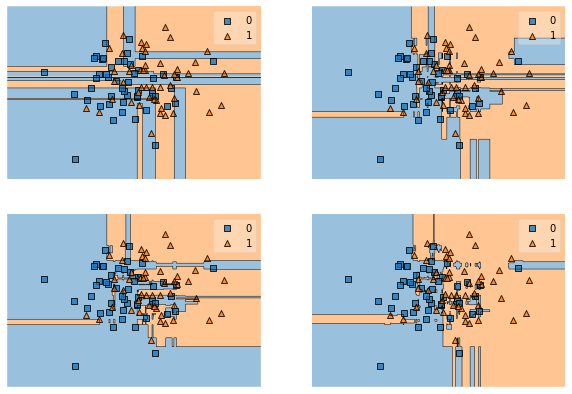
\includegraphics[scale=0.7]{rf_var1.png}
\end{center}

\end{question}

\newpage 



\section*{Часть третья: задачки}

Решите все задания. Все ответы должны быть обоснованы. Решения должны быть прописаны для каждого пункта. Рисунки должны быть чёткими и понятными. Все линии должны быть подписаны. За решение каждой задачи вы можете получить до 10 баллов.
\begin{question}
После второго скандального развода Росса Моника, Чендлер, Рейчел, Фиби и Джоуи спорят, каковы шансы, что Росс разведется и в третий раз. 
$y$ - это прогноз каждого из друзей, где "1" - развод, а "0" - долгая и счастливая жизнь. Росс знает, какие признаки используют друзья. Он хочет обучить случайный лес, прогнозирующий по этим данным, разведется ли он в следующем браке или нет. Возможно, он сможет поработать над собой и снизить вероятность третьего развода.

\begin{center}
    \begin{tabular}{ccccc}
        \toprule
        $y$ & $f_1$ & $f_2$ & $f_3$ & $f_4$ \\
        \midrule
        $1$ & $5$ & $7$ & $6$ & $9$\\
        $1$ & $3$ & $1$ & $8$ & $9$\\
        $0$ & $0$ & $0$ & $0$ & $5$\\
        $0$ & $1$ & $1$ & $4$ & $7$\\
        $1$ & $2$ & $4$ & $3$ & $2$\\
        \bottomrule
    \end{tabular}
\end{center}


Обучите 5 деревьев глубины 1. Используйте Accuracy в качестве критерия разбиения.
Для каждого дерева используйте следующие пары признаков для поиска наилучшего разбиения:

\begin{table}[h]
    \centering
    \begin{tabular}{>{\bfseries}ccc}
        \toprule
        Номер & Признак 1 & Признак 2 \\ \midrule
         Дерево 1 & $f_1$ & $f_2$\\ 
         Дерево 2 & $f_2$ & $f_4$\\ 
         Дерево 3 & $f_2$ & $f_3$\\
         Дерево 4 & $f_1$ & $f_3$\\ 
         Дерево 5 & $f_3$ & $f_4$\\ 
    \end{tabular}
\end{table}

Сделайте прогноз для нового объекта с признаками $(3, 5, 0, 6)$


\end{question}

\newpage 

\begin{question}
Рейчел прочитала в Vogue, что все модные дома используют технологии машинного обучения. Она решила отсортировать склад одежды в магазине, где работает, на две части, пользуясь методом k-means. Помогите Рейчел рассортировать одежду! Стартовые центры кластеров заданы треугольниками.
\begin{center}
    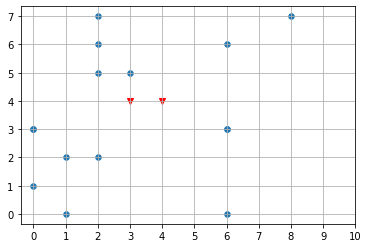
\includegraphics[scale=0.5]{k_means_var1.png}
\end{center}
\end{question}


\end{document}

